%%%%%%%%%%%%%%%%%%%%%%%%%%%%%%%%%%%%%%%%%%%%%%%%%%%%%%%%%%%
% --------------------------------------------------------
% Tau
% LaTeX Template
% Version 2.4.4 (28/02/2025)
%
% Author: 
% Guillermo Jimenez (memo.notess1@gmail.com)
% 
% License:
% Creative Commons CC BY 4.0
% --------------------------------------------------------
%%%%%%%%%%%%%%%%%%%%%%%%%%%%%%%%%%%%%%%%%%%%%%%%%%%%%%%%%%%

\documentclass[9pt,a4paper,column,twoside]{tau-class/tau}
\usepackage[english]{babel}

%% Spanish babel recomendation
% \usepackage[spanish,es-nodecimaldot,es-noindentfirst]{babel} 

%% Draft watermark
% \usepackage{draftwatermark}

%----------------------------------------------------------
% TITLE
%----------------------------------------------------------

\journalname{Intro Microelectronic Circuits with Laboratory}
\title{A Current-Mirror Differential Amplifier}

%----------------------------------------------------------
% AUTHORS, AFFILIATIONS AND PROFESSOR
%----------------------------------------------------------

\author[1]{Henry Tejada Deras}
\author[1]{Elias Tuthill}

%----------------------------------------------------------

\affil[1]{Franklin W. Olin College of Engineering}

%----------------------------------------------------------
% FOOTER INFORMATION
%----------------------------------------------------------

\institution{Franklin W. Olin College of Engineering}
\footinfo{Intro Microelectronic Circuits with Laboratory}
\theday{TBD}
\leadauthor{Tejada Deras et. al.}

%----------------------------------------------------------

\begin{document}
		
    \maketitle 
    \thispagestyle{firststyle} 
    % \tauabstract 
    % \tableofcontents
    % \linenumbers 
    
%----------------------------------------------------------

\section{Voltage Transfer Characteristics}
    \subsection{Results}
    \begin{figure}[H]
        \centering
        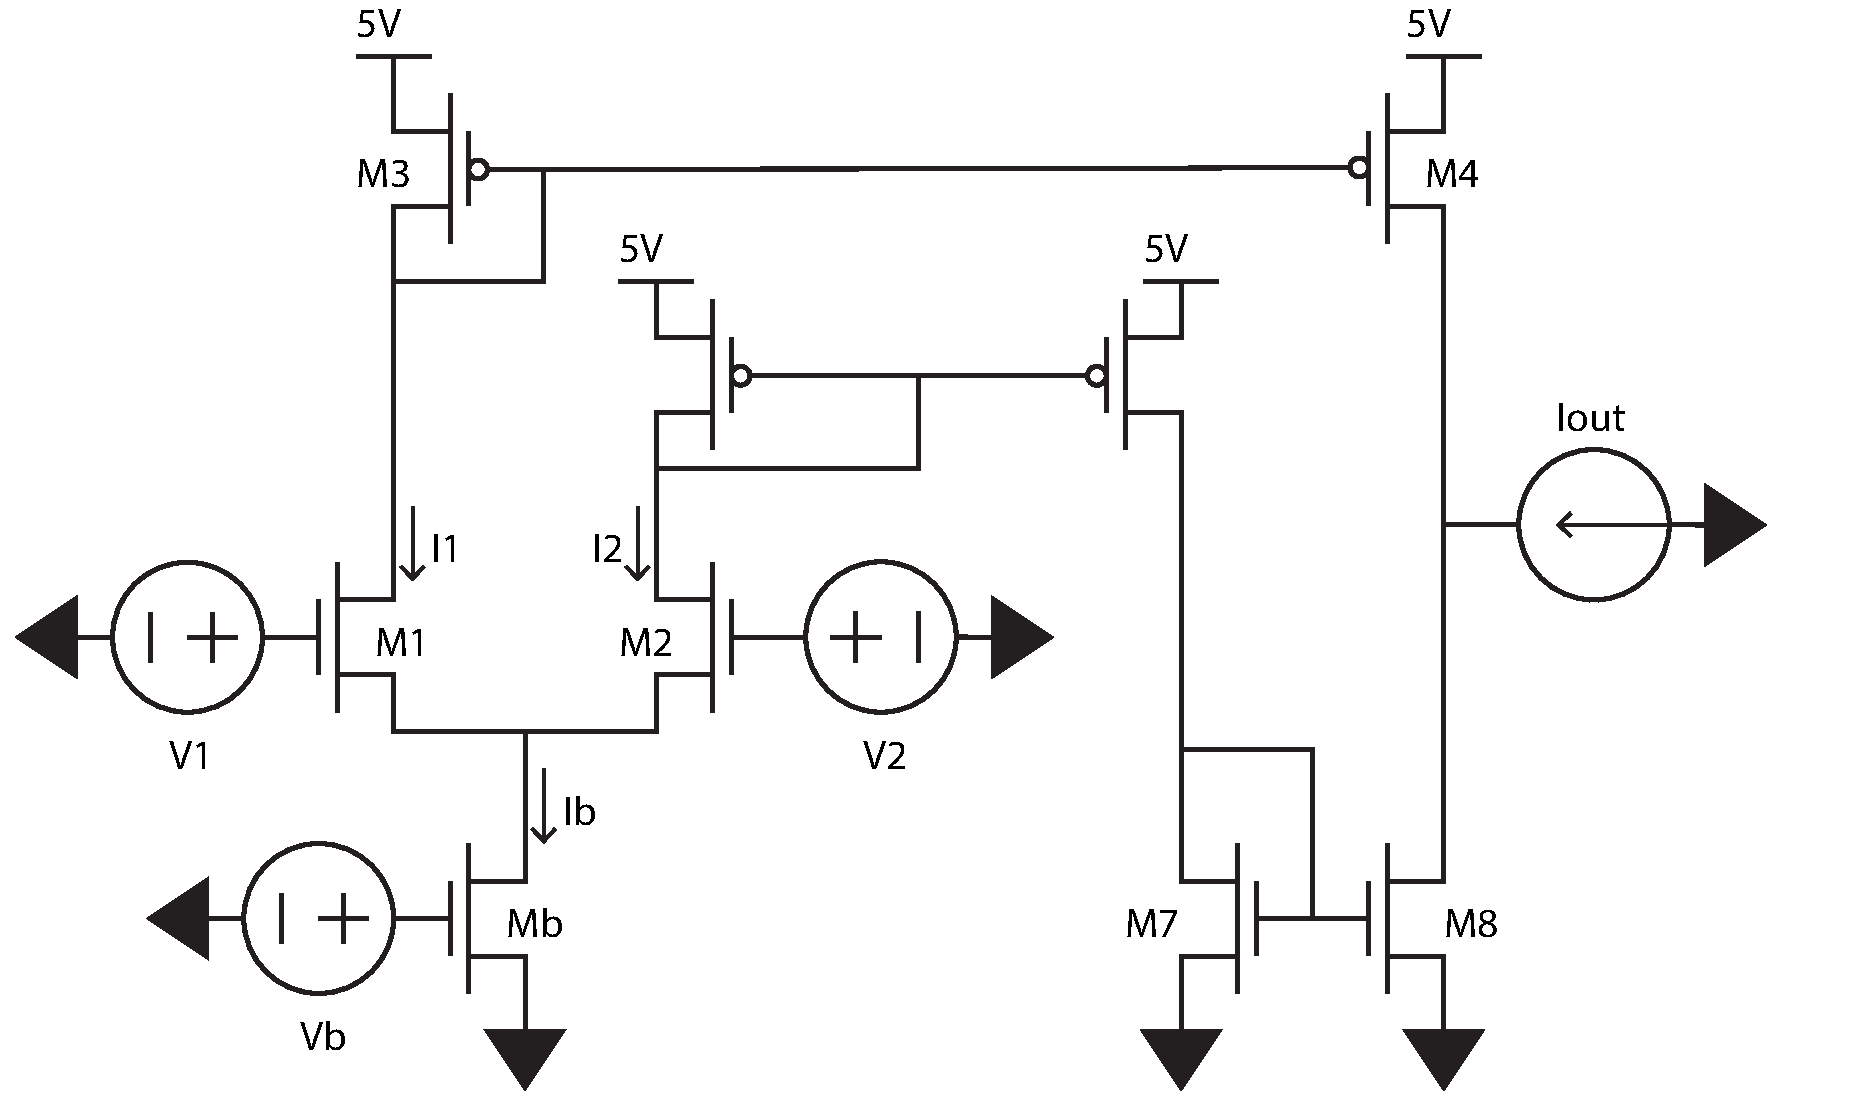
\includegraphics[width=0.6\linewidth]{../diagrams/lab7_exp1_diagram.pdf}
        \caption{Schematic of the current-mirror differential amplifier used for Voltage Transfer Characteristic (VTC) measurements.}\label{fig:exp1_diagram}
    \end{figure}

    \begin{figure}[H]
        \centering
        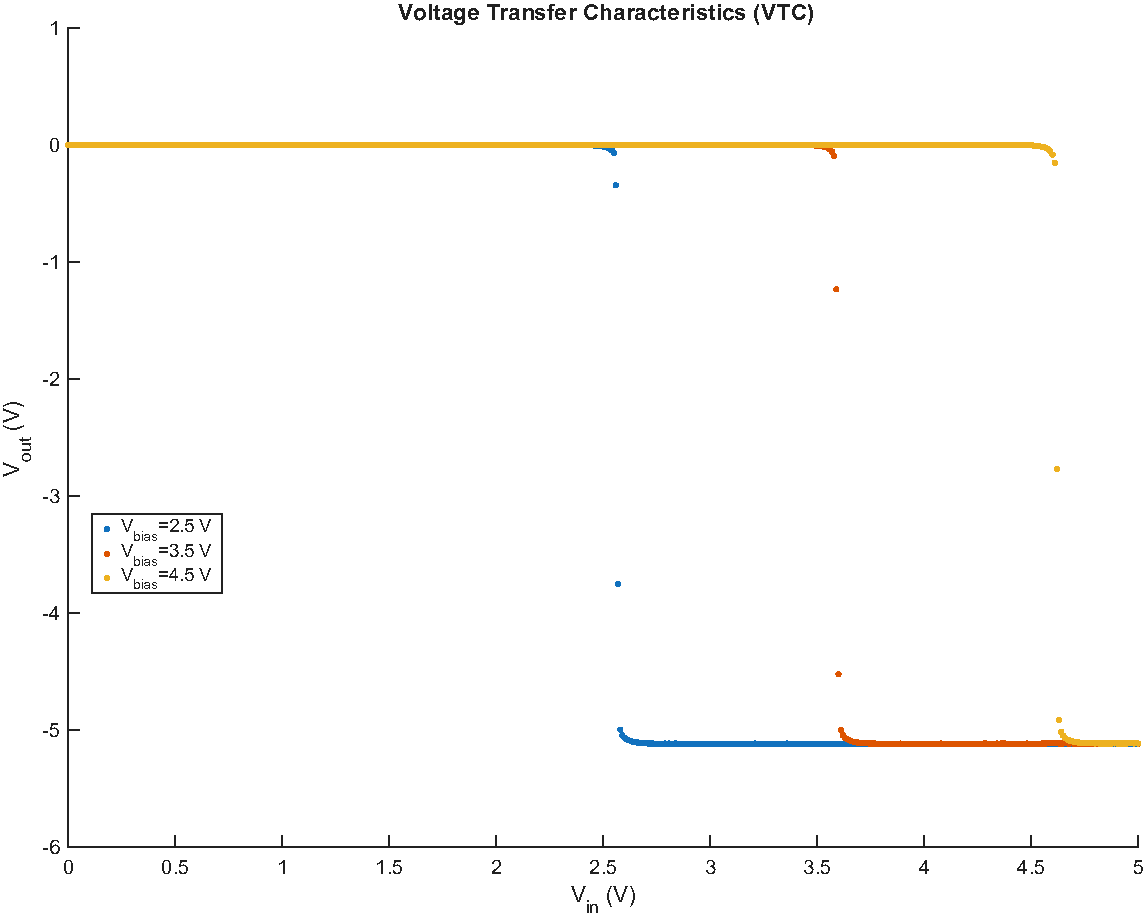
\includegraphics[width=0.6\linewidth]{../diagrams/lab7_exp1_vtc.pdf}
        \caption{Voltage Transfer Characteristics (VTC) of the current-mirror differential amplifier. The plot shows the output voltage ($V_{out}$) versus the input voltage ($V_{in}$) for three different inverting input bias voltages: $V_{bias} = 2.5$ V, $3.5$ V, and $4.5$ V.}\label{fig:exp1_vtc}
    \end{figure}

    \subsection{Analysis}
    \subsection{Discussion}

\section{Transconductance, Output Resistance, and Gain}
    \subsection{Results}
    \begin{figure}[H]
        \centering
        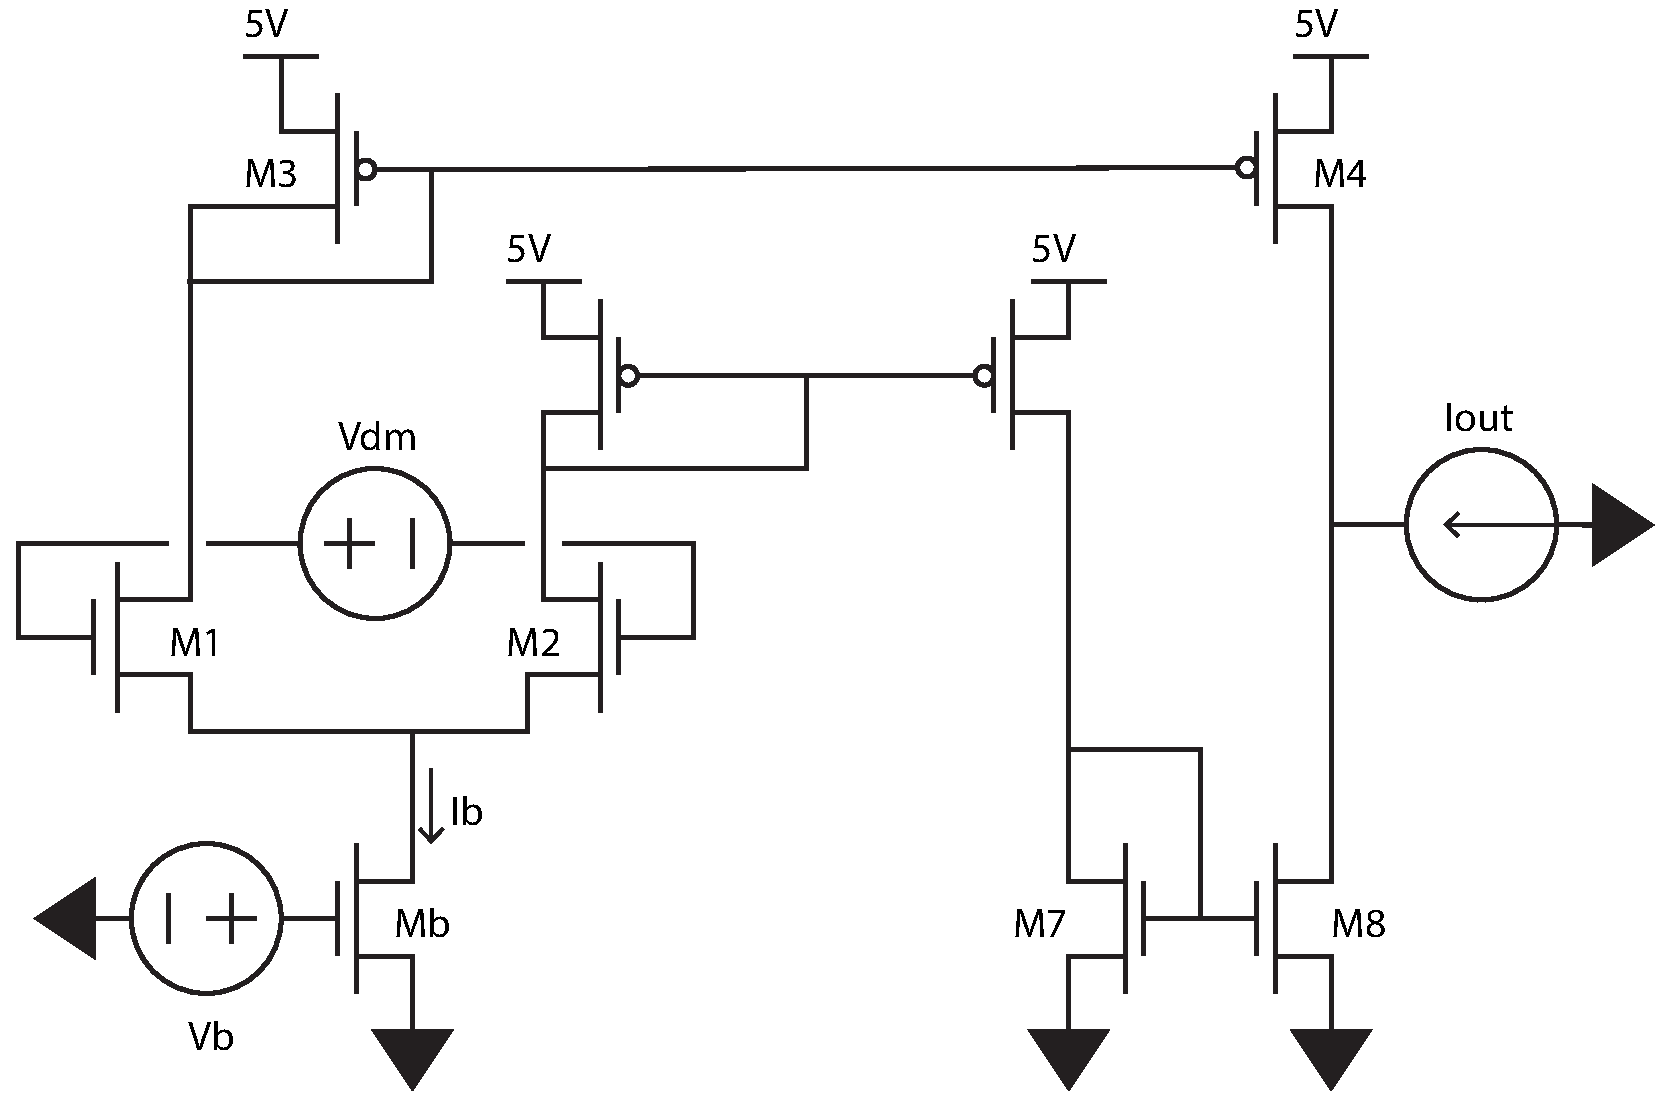
\includegraphics[width=0.6\linewidth]{../diagrams/lab7_exp2_1_diagram.pdf}
        \caption{Schematic for differential-mode voltage gain measurement.}\label{fig:exp2_diagram_gain}
    \end{figure}

    \begin{figure}[H]
        \centering
        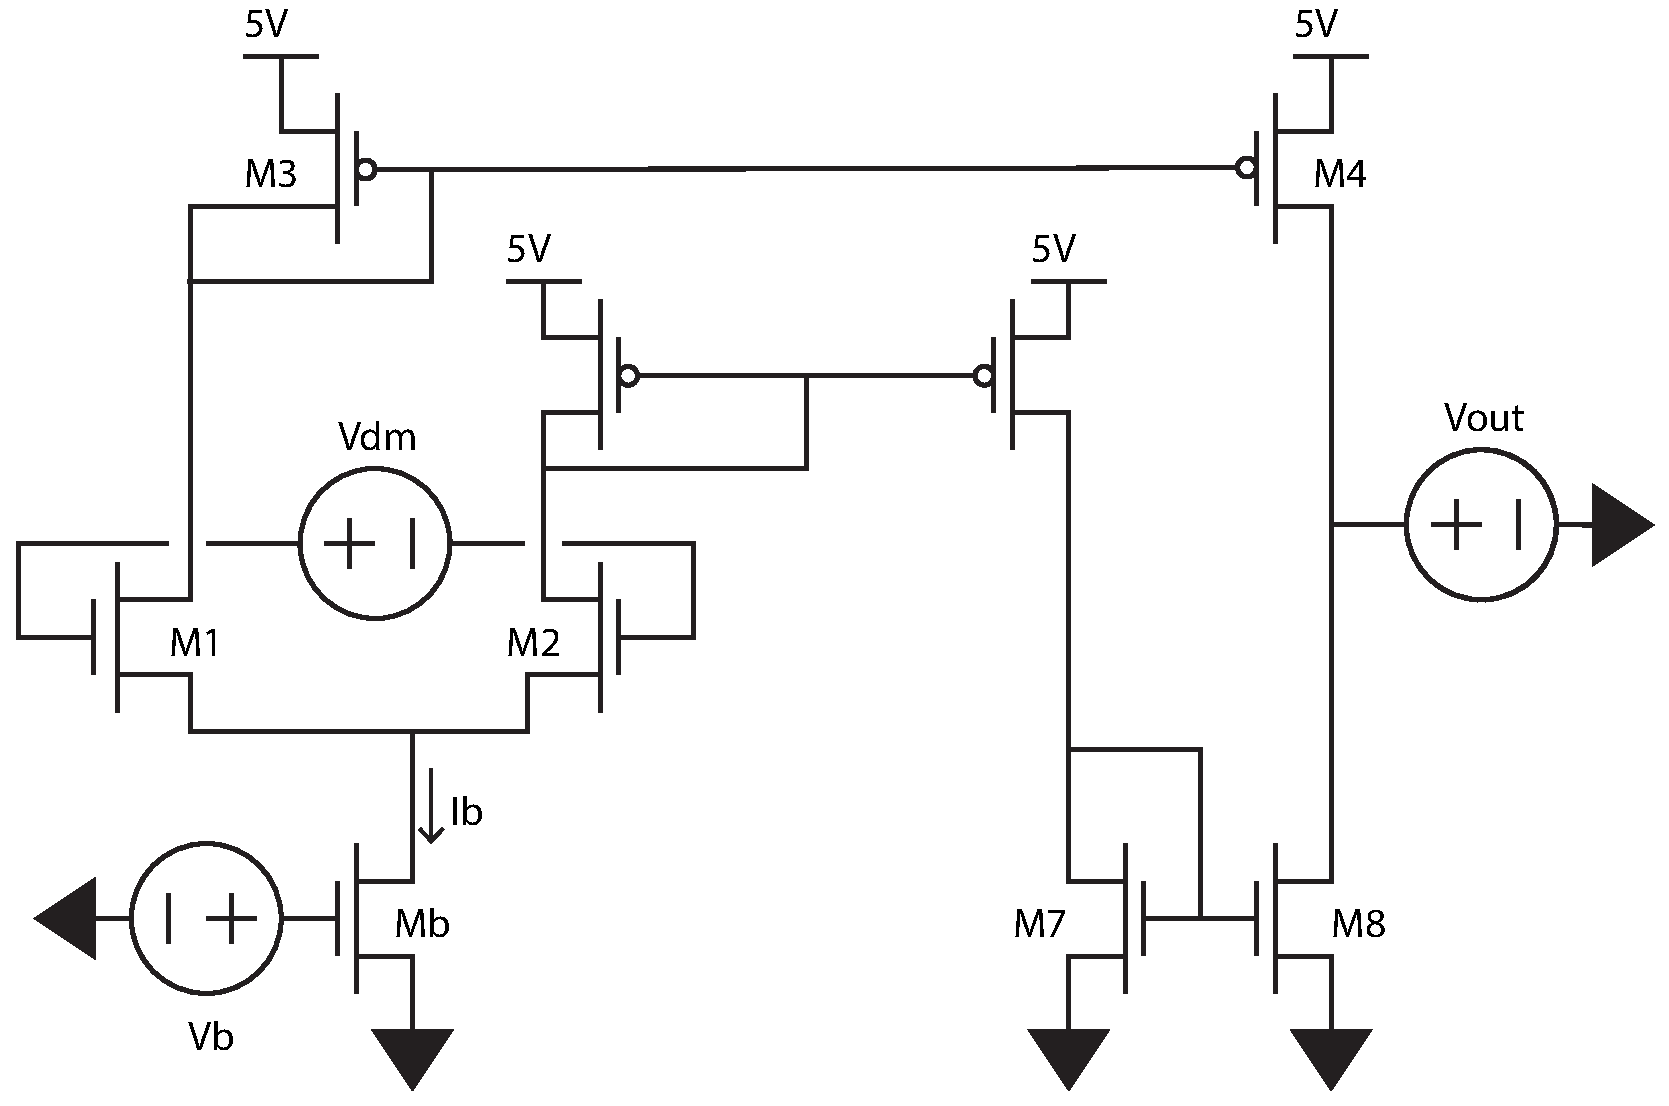
\includegraphics[width=0.6\linewidth]{../diagrams/lab7_exp2_23_diagram.pdf}
        \caption{Schematic used for both incremental transconductance ($g_m$) and output resistance ($r_{out}$) measurements.}\label{fig:exp2_diagram_shared}
    \end{figure}

    \begin{figure}[H]
        \centering
        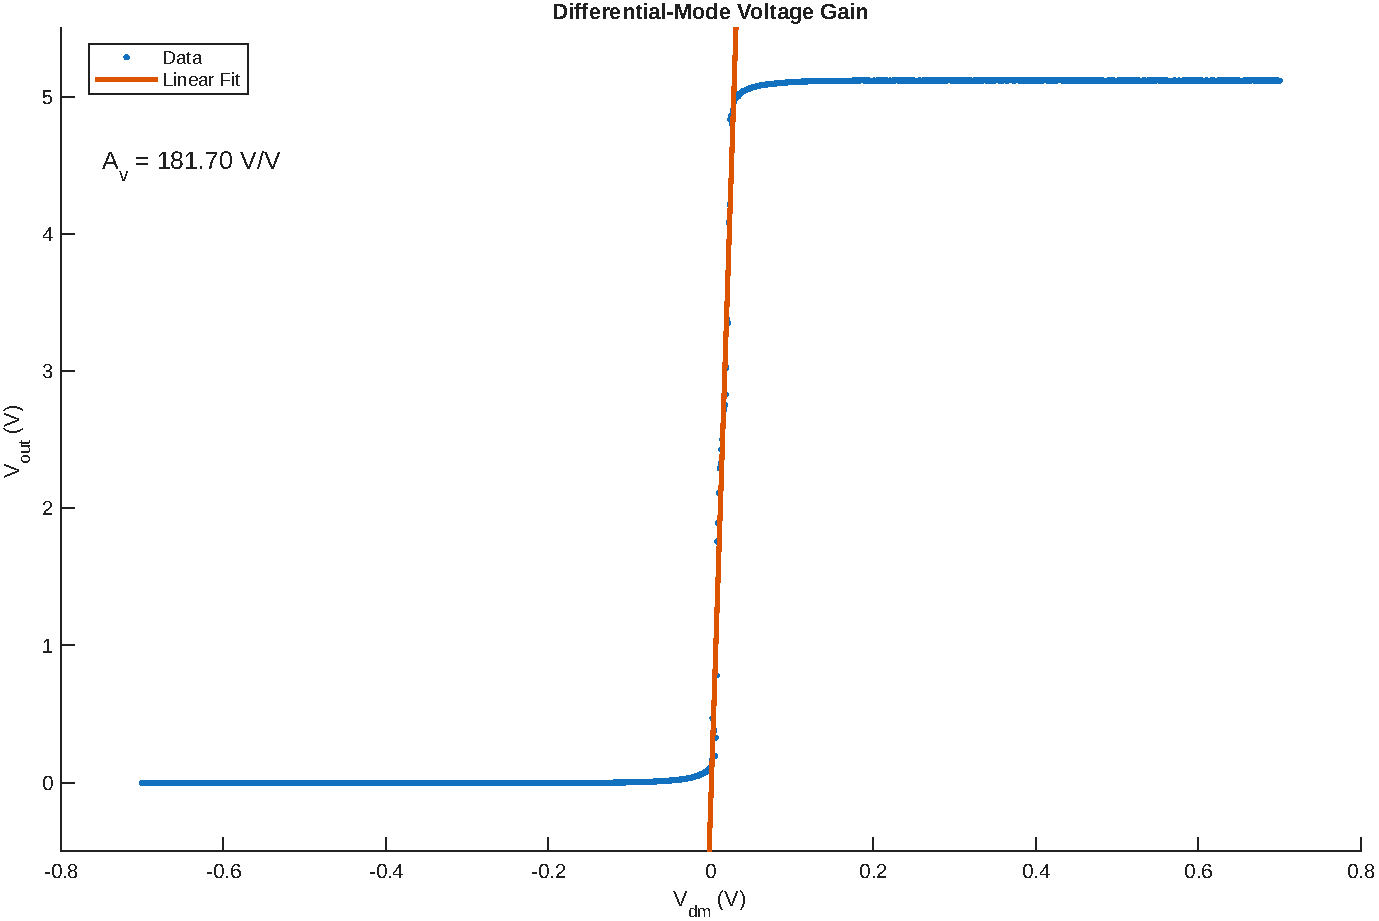
\includegraphics[width=0.6\linewidth]{../diagrams/lab7_exp2_gain.pdf}
        \caption{Differential-mode voltage gain measurement showing the output voltage ($V_{out}$) versus the differential input voltage ($V_{dm}$). A linear fit to the high-gain region gives a voltage gain of $A_v = 181.70$ V/V.}\label{fig:exp2_gain}
    \end{figure}

    \begin{figure}[H]
        \centering
        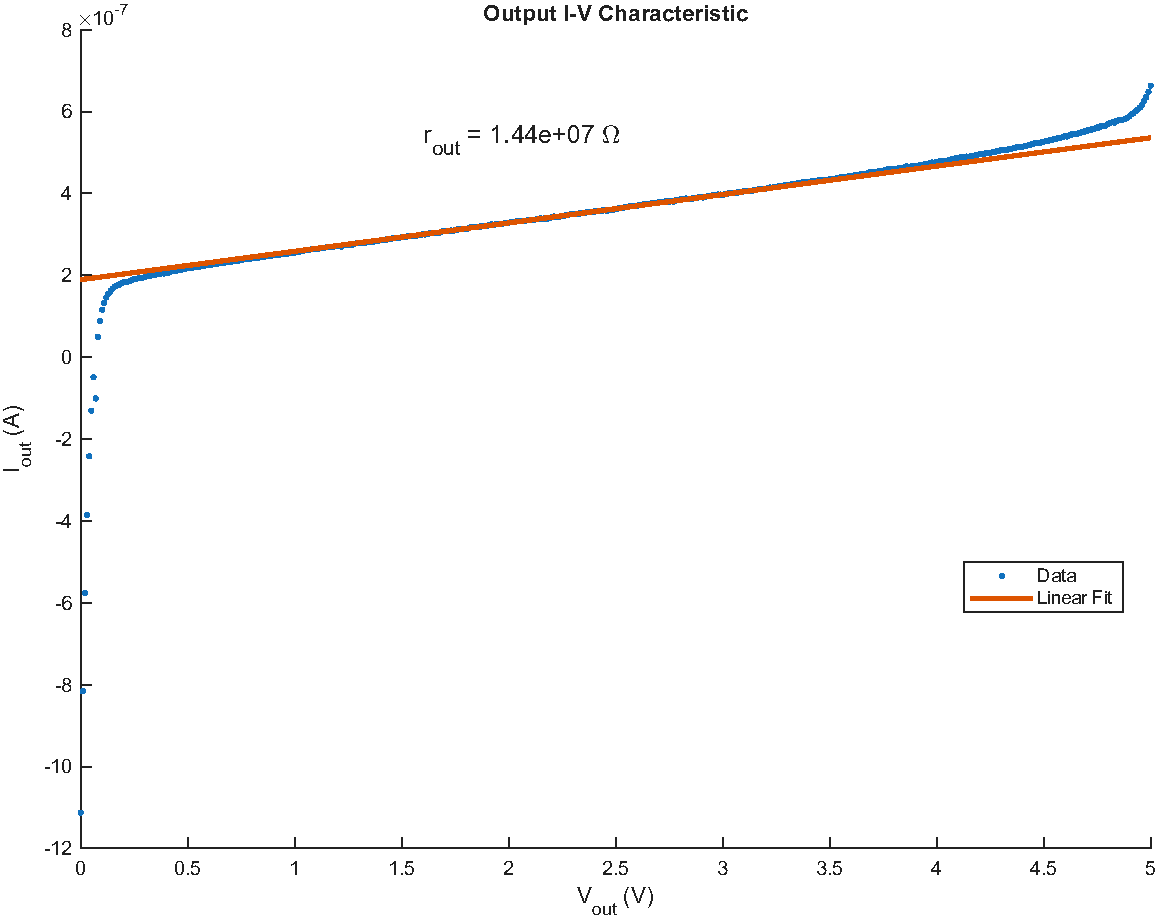
\includegraphics[width=0.6\linewidth]{../diagrams/lab7_exp2_iv.pdf}
        \caption{Output current-voltage characteristic curve showing $I_{out}$ versus $V_{out}$ with $V_{dm} = 0$ V. The inverse slope of the linear fit gives an incremental output resistance of $r_{out} = 1.44 \times 10^7 \ \Omega$.}\label{fig:exp2_iv}
    \end{figure}

    \begin{figure}[H]
        \centering
        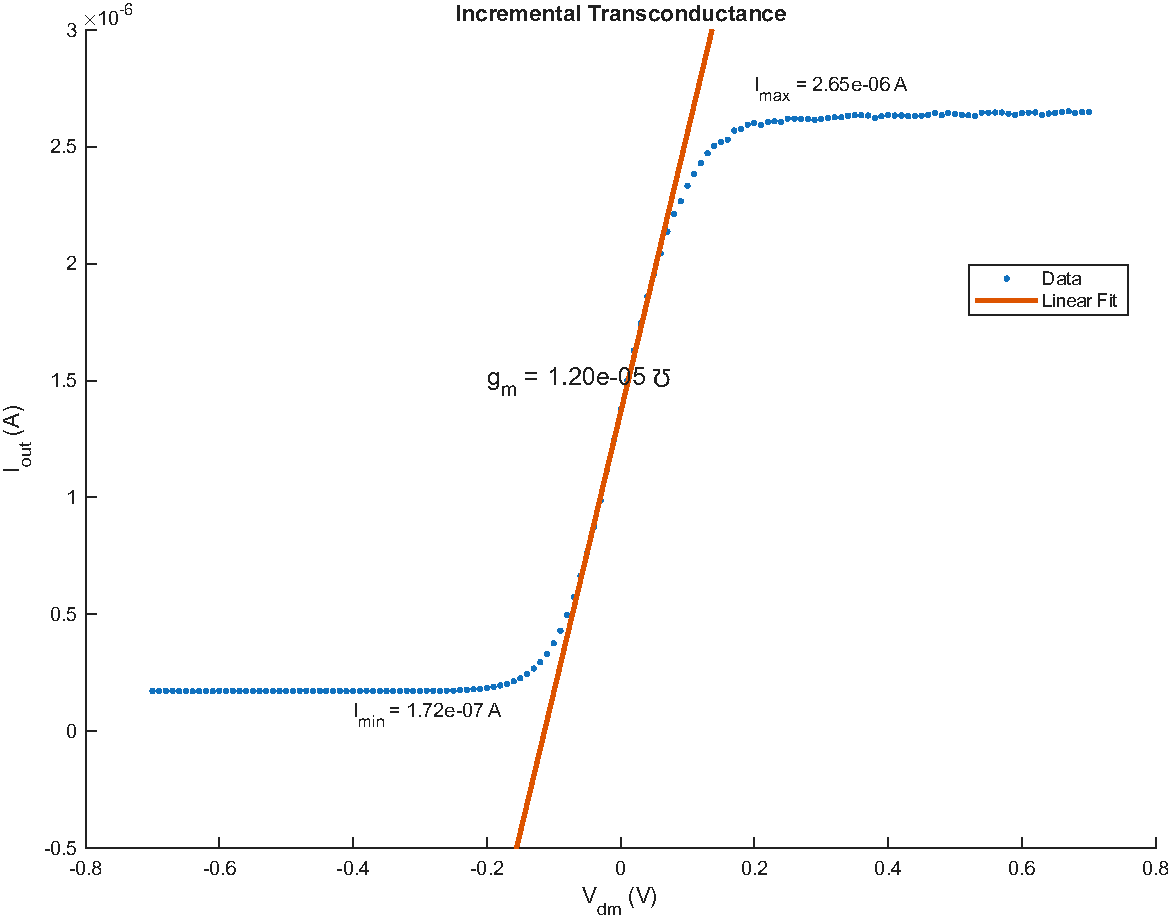
\includegraphics[width=0.6\linewidth]{../diagrams/lab7_exp2_itranscon.pdf}
        \caption{Incremental transconductance measurement showing the output current ($I_{out}$) versus the differential input voltage ($V_{dm}$) with a fixed output voltage. The linear fit gives a transconductance of $g_m = 1.20 \times 10^{-5} \ \Omega^{-1}$.}\label{fig:exp2_transcon}
    \end{figure}


    \subsection{Analysis}
    \subsection{Discussion}
\section{Unity-Gain Follower Step Response}
    \subsection{Results}

	
\begin{figure}[H]
        \centering
        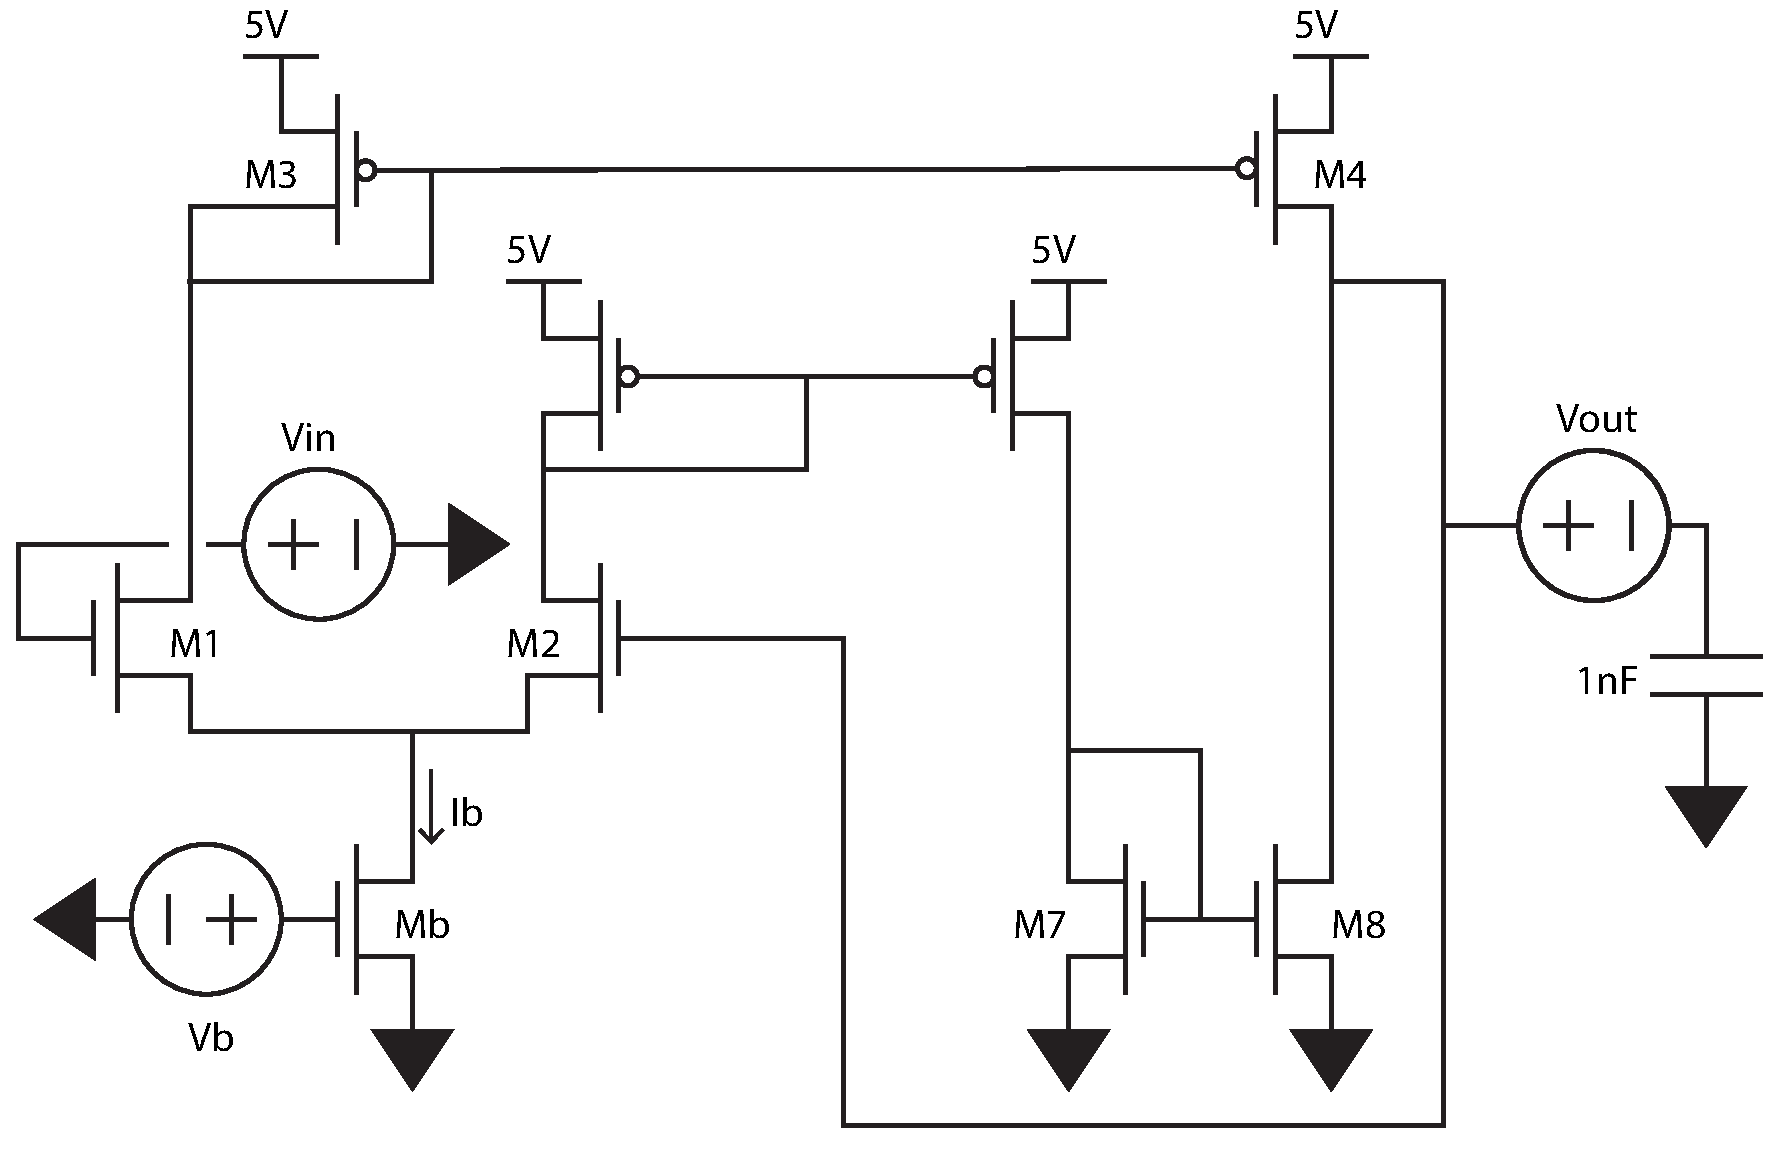
\includegraphics[width=0.6\linewidth]{../diagrams/lab7_exp3_diagram.pdf}
        \caption{Schematic of the current-mirror differential amplifier used as a unity-gain follower (buffer) driving a 1 nF load capacitor.}\label{fig:exp3_setup}
    \end{figure}

    \begin{figure}[H]
        \centering
        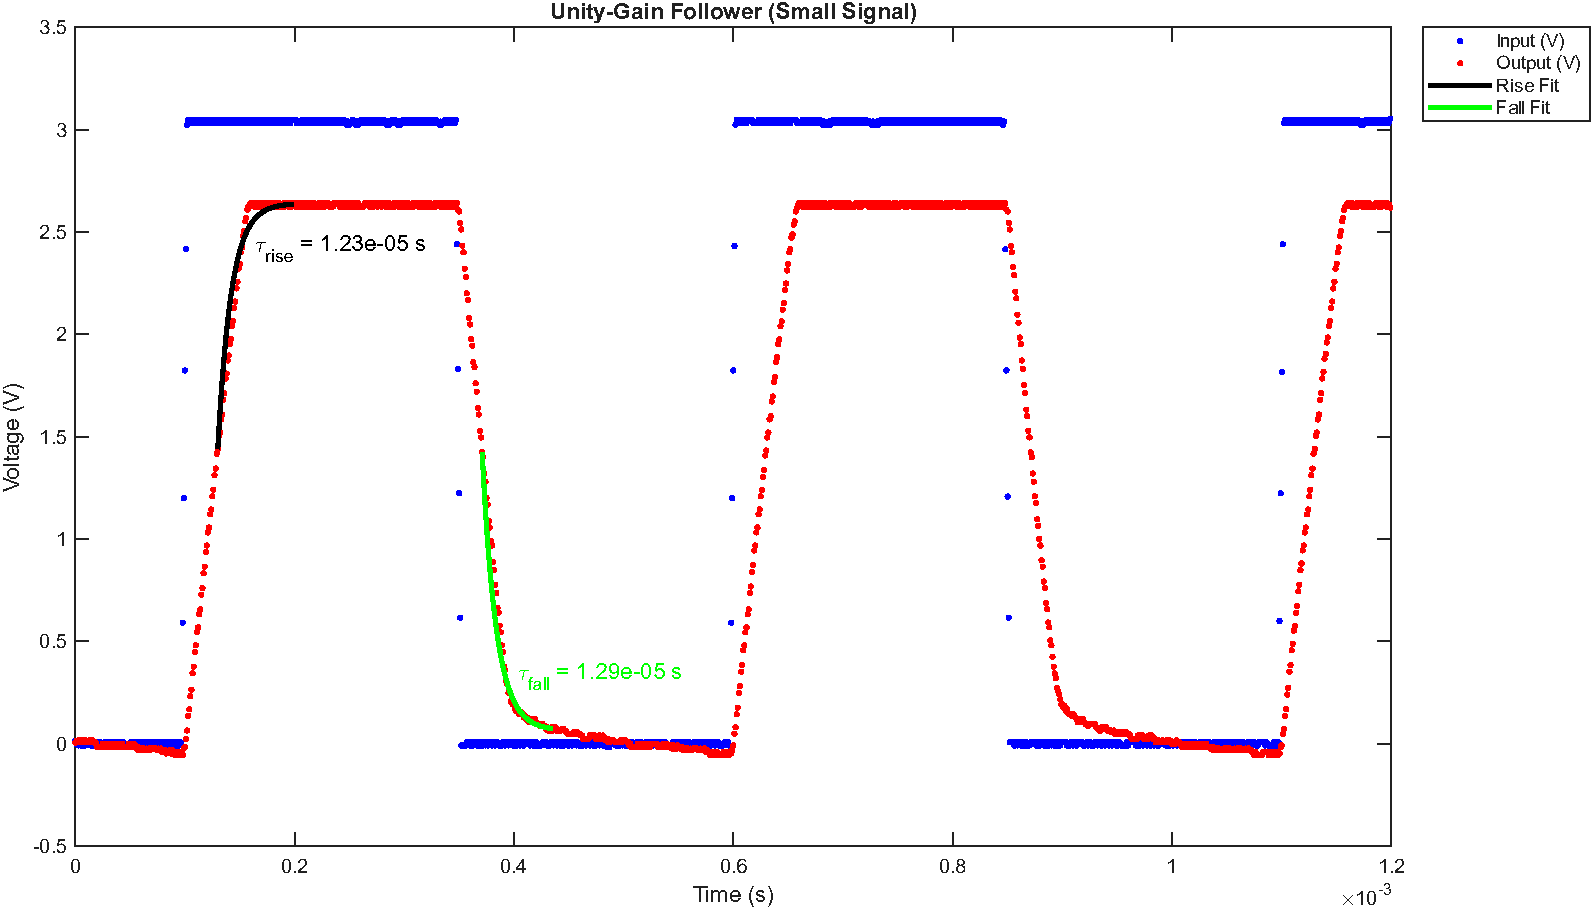
\includegraphics[width=0.8\linewidth]{../diagrams/lab7_exp3_1.pdf}
        \caption{Small signal step response of the current-mirror differential amplifier as a unity-gain follower driving a 1 nF load capacitor. Extracted rise and fall time constants are shown.}\label{fig:exp3_small_signal}
    \end{figure}

    
    \begin{figure}[H]
        \centering
        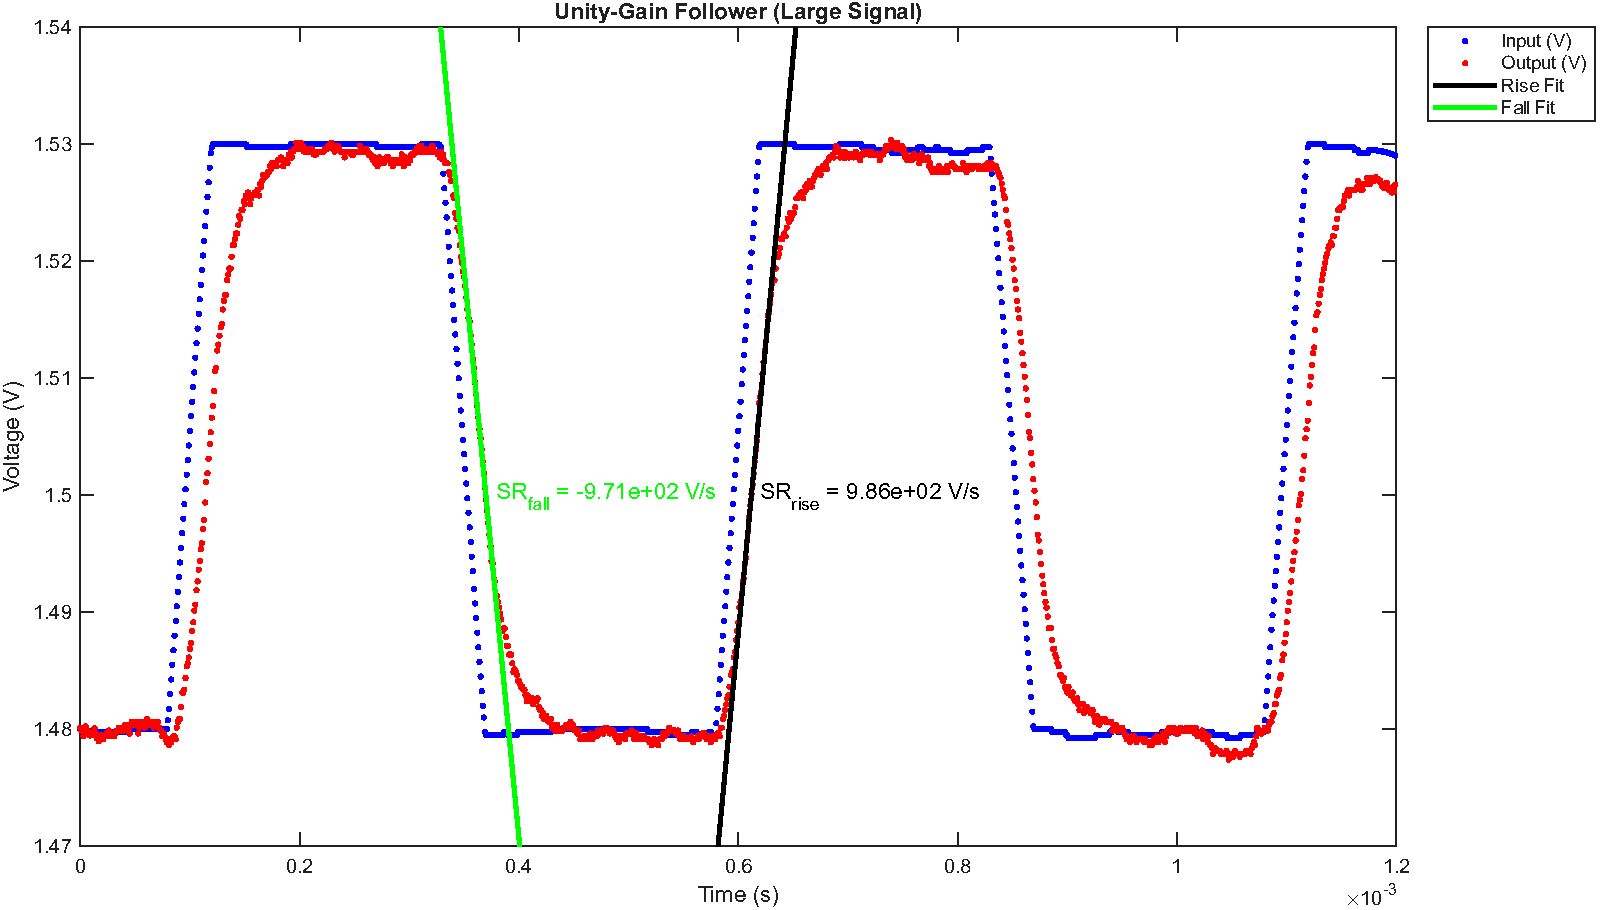
\includegraphics[width=0.8\linewidth]{../diagrams/lab7_exp3_large.pdf}
        \caption{Large signal step response of the unity-gain follower configuration, showing linear slewing. The positive and negative slew rates (SR) are labeled.}\label{fig:exp3_large_signal}
    \end{figure}

    \subsection{Analysis}
    \subsection{Discussion}
%----------------------------------------------------------

\end{document}